\documentclass[10pt,a4paper]{article}

% ── packages ──────────────────────────────────────────────────────────────────
\usepackage{amsmath,amssymb}
\usepackage{booktabs}
\usepackage{graphicx}
\usepackage{hyperref}
\usepackage{multirow}
\usepackage{microtype}
\usepackage{geometry}
\usepackage{natbib}
\usepackage{xcolor}
\geometry{margin=1in}

\hypersetup{
    colorlinks=true,
    linkcolor=blue!70!black,
    citecolor=green!50!black,
    urlcolor=blue,
}

% ── document ──────────────────────────────────────────────────────────────────
\begin{document}

\title{Thermodynamic Continual Learning: Activation Entropy Governs Catastrophic Forgetting}
\author{\textbf{Christopher Gardner} \\\\ \small Independent Research}
\date{May 2026}
\maketitle

\begin{abstract}
Continual learning methods are commonly evaluated on a single scalar: catastrophic
forgetting. We show this metric has a systematic failure mode --- importance-weighted
regularisation methods can achieve low forgetting scores while producing networks that
have learned nothing, by collapsing to chance-level predictions on every task.

We introduce Thermodynamic Continual Learning (TCL), a method that uses per-task
activation entropy as a consolidation signal to govern weight regularisation during
sequential learning. TCL anchors a reference entropy $\sigma^\star$ from the first
task batches and detects the ordered regime (consolidation) when the running entropy
falls below this reference, triggering a dimensionality-weighted L2 anchor penalty.

On Split-CIFAR-10 with a ResNet-18 backbone across five random seeds, TCL achieves
mean forgetting $0.1161 \pm 0.029$ against SGD's $0.2331 \pm 0.003$
($\Delta = -0.1170$, $p = 0.0012$, Cohen's $d = 3.68$, 5/5 seeds TCL
better) and EWC at its published default ($\lambda = 100$) $0.1909 \pm 0.023$
($\Delta = -0.0748$, $p = 0.0190$, Cohen's $d = 1.70$, 5/5 seeds TCL
better). A penalty-strength sweep reveals that appropriately tuned EWC
($\lambda = 1000$) achieves $0.1602 \pm 0.089$, not significantly different from TCL
($p = 0.318$); TCL's advantage is that it requires no hyperparameter search to reach
this performance level. Well-tuned SI ($c = 0.01$) achieves lower forgetting
($0.0488 \pm 0.009$) than TCL, at the cost of requiring careful calibration: at
published defaults ($c = 0.1$), SI collapses to $0.500$ accuracy on all five seeds,
demonstrating the failure mode of forgetting-only evaluation.
A pre-registered ablation shows the L2 anchor penalty is the primary mechanistic
component: governor-only tracks SGD, while penalty-only captures most of the
forgetting reduction (full TCL $0.1272 \pm 0.022$ vs.~penalty-only
$0.1429 \pm 0.018$; full-vs.-penalty gap not yet resolved at $n=5$,
$p = 0.3154$, $d = 0.51$). We propose the joint accuracy-forgetting (JAF) metric as
a minimal two-dimensional reporting standard that exposes degenerate solutions
invisible to forgetting-only evaluation. A scale-up to Split-TinyImageNet
(10 tasks, 3 seeds) confirms the SGD reduction transfers to a harder benchmark:
TCL achieves mean forgetting $0.0221 \pm 0.006$ vs.\ SGD's $0.5183 \pm 0.011$
($\Delta = -0.4962$, $p = 0.0001$, $d = 75.1$, 3/3 seeds); the TCL vs.\ EWC
comparison is not resolved at $n = 3$ ($p = 0.359$).
\end{abstract}

\tableofcontents
\newpage

\section{Introduction}
\label{sec:introduction}

Neural networks trained sequentially on multiple tasks suffer from catastrophic
forgetting: gradient updates that adapt the network to a new task systematically
overwrite the weight configurations that encoded prior tasks, leading to abrupt
performance collapse on earlier data~\cite{McCloskey1989}.
This phenomenon is not a mere implementation detail but a structural consequence
of shared parameter spaces and unconstrained gradient descent; a network that
achieves near-perfect performance on Task~$T$ after learning Task~$T{+}1$ will
frequently revert to chance-level accuracy on~$T$, as though the earlier training
had never occurred~\cite{Kirkpatrick2017}.
The severity of the problem scales with task dissimilarity and network depth,
making it a fundamental obstacle to deploying neural networks in settings where
the data distribution shifts over time.

Existing regularisation-based approaches address catastrophic forgetting by
penalising changes to parameters judged important for previous tasks.
Elastic Weight Consolidation (EWC) computes a Fisher information matrix after
each task and uses its diagonal as a per-parameter importance weight in a
quadratic penalty term~\cite{Kirkpatrick2017}.
Synaptic Intelligence (SI) accumulates an online surrogate importance measure
by tracking the contribution of each parameter to the loss reduction throughout
training~\cite{Zenke2017}.
Both methods share the requirement of maintaining and updating a full set of
per-parameter importance weights, which adds memory and computation overhead
proportional to the number of learnable parameters.
A more subtle and empirically consequential failure mode, however, lies in the
interaction between importance weighting and network calibration: when importance
weights are over-constraining, the network can be driven into a degenerate
solution in which it outputs a constant prediction for all inputs, collapsing
to chance-level accuracy on every task while still satisfying the forgetting
penalty.
Under forgetting-only evaluation this collapse is invisible, because a network
that has never moved from its initial prediction incurs zero measurable forgetting.
This asymmetry between forgetting metrics and accuracy motivates a two-dimensional
evaluation standard.

We propose Thermodynamic Continual Learning (TCL), a method that replaces
per-parameter importance estimation with a coarser, thermodynamically motivated
consolidation signal derived from the activation distribution of the network
during task training.
TCL monitors the \emph{thermal ratio} $\rho = \sigma / \sigma^\star$, where
$\sigma$ is the current standard deviation of task-specific activations and
$\sigma^\star$ is a reference value estimated at the beginning of training.
When $\rho < 0.9$---indicating that the activation distribution has contracted
into an ordered, low-entropy regime---TCL applies a $D_\text{PR}$-weighted
$\ell_2$ anchor penalty that constrains the network weights to remain close to
their values at the consolidation moment.
When $\rho \geq 0.9$, the network is in a disordered regime and the penalty is
not applied.
Crucially, TCL requires no Fisher matrix computation and no per-parameter
importance bookkeeping: the consolidation decision is made thermodynamically,
from aggregate activation statistics, rather than from gradient statistics.

The contributions of this paper are threefold.
\begin{enumerate}
  \item \textbf{The TCL method.}
        We introduce an activation-entropy-driven thermodynamic governor
        that detects the consolidation moment via the thermal ratio $\rho$
        and applies a $D_\text{PR}$-weighted $\ell_2$ anchor penalty when the
        ordered regime is entered.
        The method is parameter-light, requires a single scalar threshold,
        and adds no per-parameter storage.

  \item \textbf{Empirical results with honest baseline comparison.}
        TCL reduces forgetting significantly versus SGD ($\Delta = -0.1170$,
        $p = 0.0012$, $d = 3.68$, 5/5 seeds) and default EWC
        ($\Delta = -0.0748$, $p = 0.0190$, $d = 1.70$, 5/5 seeds).
        A penalty-sweep (Appendix~\ref{app:ewc-sweep}) shows that tuned EWC
        ($\lambda = 1000$) is not significantly different from TCL ($p = 0.318$);
        well-tuned SI ($c = 0.01$) achieves lower forgetting than TCL.
        TCL's advantage is that it requires no penalty hyperparameter to reach
        competitive performance.
        A component ablation (Section~\ref{sec:ablation}) shows the anchor penalty
        is the load-bearing element; the governor's marginal contribution is
        directional but unresolved at $n = 5$ ($p = 0.315$).

  \item \textbf{The JAF (joint accuracy-forgetting) metric.}
        We propose JAF (Eq.~\ref{eq:jaf}) as a minimal two-dimensional evaluation
        standard that exposes degenerate solutions invisible to forgetting-only
        metrics.
        At published defaults ($c = 0.1$), SI collapses to $0.500$ accuracy on all
        five seeds while reporting competitive forgetting scores, because a constant-output
        network incurs zero measurable forgetting.
        A robustness sweep (Section~\ref{sec:si-robustness}) shows this failure is
        specific to part of the default neighbourhood: $c = 0.01$ recovers non-trivial
        accuracy, whereas $c \in \{0.1, 0.5\}$ remains collapsed.
\end{enumerate}

The remainder of this paper is organised as follows.
Section~\ref{sec:background} reviews the continual learning literature,
the thermodynamic analogy, and the evaluation protocols that motivate JAF.
Section~\ref{sec:method} presents the TCL algorithm, the $\rho$ governor,
the $D_\text{PR}$-weighted anchor penalty, and the JAF metric definition.
Section~\ref{sec:experiments} reports the primary four-way comparison
(Section~\ref{sec:baseline}), a component ablation (Section~\ref{sec:ablation}),
an SI robustness sweep (Section~\ref{sec:si-robustness}), and a scale-up to
Split-TinyImageNet (Section~\ref{sec:tinyimagenet}).
Section~\ref{sec:discussion} interprets the results, discusses limitations
including the class-incremental scope boundary, and situates TCL within the
broader continual learning landscape.
Section~\ref{sec:conclusion} summarises the contributions and outlines future work.
Appendix~\ref{app:ewc-sweep} reports the EWC penalty-strength sweep;
Appendix~\ref{app:reproducibility} provides full reproducibility details.


% s2_background.tex
% Status: DRAFT — generated by TAR-Author; review before locking
% Lock condition: after related work citations verified

\section{Background and Related Work}
\label{sec:background}

\subsection{Catastrophic Forgetting and Continual Learning Scenarios}

Catastrophic forgetting~\cite{McCloskey1989} is the tendency of neural networks to
lose performance on previously learned tasks when trained sequentially on new ones.
The problem arises because stochastic gradient descent updates weights to minimise
loss on the current task without preserving knowledge of prior tasks.
\citet{vandeVen2019} distinguish three evaluation scenarios: \emph{task-incremental}
(task identity provided at test time), \emph{domain-incremental} (task identity
hidden but output space fixed), and \emph{class-incremental} (task identity hidden
and output space grows).
This paper addresses the task-incremental scenario exclusively; as reported in
Section~\ref{sec:discussion}, the current TCL architecture does not resolve the
class-incremental case.

\subsection{Regularisation-Based Continual Learning}

Elastic Weight Consolidation (EWC)~\cite{Kirkpatrick2017} penalises changes to
weights identified as important using the diagonal Fisher Information Matrix as a
per-parameter importance proxy.
The penalty strength $\lambda$ governs the plasticity-stability trade-off:
insufficient $\lambda$ allows forgetting; excessive $\lambda$ can collapse the
network to degenerate predictions, as our $\lambda$-sweep (Appendix~\ref{app:ewc-sweep})
confirms.
Synaptic Intelligence (SI)~\cite{Zenke2017} estimates weight importance online by
accumulating the product of gradients and parameter changes during training.
Memory Aware Synapses (MAS)~\cite{Aljundi2018} computes importance from the
gradient of the squared $\ell_2$ output norm, removing the dependency on task labels.
All three methods share a common limitation: they maintain a full-parameter importance
vector, whose memory cost scales linearly with the number of parameters and must be
updated or consolidated after every task.
They also share a common failure mode under over-constraining penalty strength:
Section~\ref{sec:si-collapse} and Appendix~\ref{app:ewc-sweep} show that both SI
and EWC can collapse to chance-level accuracy when their penalty coefficients are
too large or poorly tuned.
TCL avoids per-parameter importance scores entirely; the only auxiliary state is the
scalar anchor $\sigma^\star_k$ and the parameter snapshot $\theta^\star_k$ per task.

\subsection{Replay-Based Methods}

Generative replay~\cite{Shin2017} trains a generative model alongside the classifier
and rehearses synthetic samples of previous tasks.
iCaRL~\cite{Rebuffi2017} stores a small exemplar set for replay and nearest-class-mean
classification.
Gradient Episodic Memory (GEM)~\cite{LopezPaz2017} constrains gradient updates to
not increase loss on stored episodic memories, with A-GEM~\cite{Chaudhry2018}
providing a more efficient approximate formulation.
Dark Experience Replay (DER++)~\cite{Buzzega2020} replays both past logits and labels,
achieving strong performance with small buffers.
All replay methods require storing past data or representations, which is prohibited
in our experimental setting; we do not compare against them, but note that TCL's
activation-entropy signal is orthogonal to replay and could in principle be combined
with it.

\subsection{Parameter Isolation and Architecture-Expanding Methods}

Progressive Neural Networks~\cite{Rusu2016} add a new column of parameters per task,
preventing forgetting by construction at the cost of growing network size.
PackNet~\cite{Mallya2018} iteratively prunes and re-trains within a fixed network,
allocating capacity per task via binary masks.
These methods trade memory efficiency for zero forgetting; TCL operates within a
fixed network and does not grow or mask parameters.

\subsection{Thermodynamic Perspectives and Activation Statistics}

Thermodynamic analogies in deep learning have a long history, from Hopfield energy
functions~\cite{Hopfield1982} to flat-minima and loss-surface thermodynamics.
More recently, activation statistics have been studied as proxies for training
dynamics: large activation variance indicates an exploratory phase, small variance
indicates convergence.
Neural Collapse~\cite{Papyan2020} formalises the terminal phase of training in terms
of activation geometry, showing that class means collapse to a simplex equiangular
tight frame.
TCL is, to our knowledge, the first method to use the \emph{ratio} of current to
anchored activation standard deviation as a real-time \emph{control signal} for
continual learning: rather than measuring importance retrospectively from gradient
statistics (as EWC and SI do), TCL detects the consolidation moment dynamically
and triggers weight anchoring at that instant.
This is qualitatively different from importance-weighting approaches and from
architecture-expanding approaches; it requires no label information, no stored
gradients, and no post-task consolidation step.


% s3_method.tex
% Status: DRAFT — generated by TAR-Author; review before locking
% Lock condition: after ablation confirmed both components are needed

\section{Method: The Thermodynamic Continual Learning Governor}
\label{sec:method}

\subsection{Notation and Thermal Ratio}

Let $\theta \in \mathbb{R}^d$ denote the network parameters and let
$a^{(\ell)}_t \in \mathbb{R}^{B \times d_\ell}$ denote the activations of layer $\ell$
at step $t$ on a batch of size $B$.
Define the \emph{thermal level} as the mean activation standard deviation across layers:
\begin{equation}
    \sigma_t = \frac{1}{L}\sum_{\ell=1}^{L} \operatorname{std}\!\left(a^{(\ell)}_t\right).
\end{equation}
At the start of task $k$, after a warmup guard of $G = 60$ batches, we record the
\emph{task anchor}:
\begin{equation}
    \sigma^\star_k = \frac{1}{W}\sum_{t=G}^{G+W-1} \sigma_t,
    \quad W = 20 \text{ batches}.
    \label{eq:anchor}
\end{equation}
The anchor is frozen for the duration of task $k$ and reset at the start of task $k+1$.
The \emph{thermal ratio} is then:
\begin{equation}
    \rho_t = \frac{\sigma_t}{\sigma^\star_k}.
    \label{eq:rho}
\end{equation}
When $\rho_t > 1$ the network is more disordered than at the anchor moment; when
$\rho_t < 1$ it has consolidated below the anchor level.

\subsection{Warmup Guard}

The warmup guard delays anchor collection until the network has settled from the
activation distribution shift that occurs at each task boundary.
Without the guard, $\sigma^\star$ reflects random-initialisation noise rather than
the network's nominal thermal level, which makes the ordered regime ($\rho < 0.9$)
unreachable in practice --- a calibration issue identified during early development.

\subsection{Regime Classification and Learning Rate Modulation}

\begin{table}[h]
\centering
\caption{Thermal regime classification and governor actions.}
\label{tab:regimes}
\begin{tabular}{llll}
\toprule
$\rho_t$ & Regime & Interpretation & LR Action \\
\midrule
$> 1.1$ & \textbf{Disordered} & Activations more variable than anchor; exploring &
    $\eta \leftarrow \eta_0\!\left(1 + \alpha(\rho_t - 1)\right)$ \\
$[0.9, 1.1]$ & \textbf{Critical} & Near equilibrium & $\eta \leftarrow \eta_0$ \\
$< 0.9$ & \textbf{Ordered} & Activations below anchor; consolidating &
    $\eta \leftarrow \eta_0\,\alpha\,\rho_t$ \\
\bottomrule
\end{tabular}
\end{table}

The interpolation coefficient $\alpha = 0.5$ is pre-registered and controls how
aggressively the governor modulates the learning rate in response to thermal state.

\subsection{Dimensionality-Weighted L2 Anchor Penalty}

When the network enters the ordered regime on task $k$, we record the parameter
vector $\theta^\star_k = \theta$ as the task weight anchor.
For all subsequent tasks $k' > k$, we add the anchor regulariser:
\begin{equation}
    \mathcal{L}_{\text{anchor}} = \lambda_{\text{TCL}} \cdot D_{\mathrm{PR}} \cdot
        \|\theta - \theta^\star_k\|^2,
    \label{eq:penalty}
\end{equation}
where $\lambda_{\text{TCL}} = 0.01$ (pre-registered) and $D_{\mathrm{PR}}$ is the
\emph{dimensionality participation ratio} --- an estimate of the effective number of
active gradient directions.
In the experiments reported here, eigenvalue decomposition is disabled for
computational efficiency (\texttt{compute\_dpr=False}), fixing $D_{\mathrm{PR}} = 1.0$;
the thermal ratio computation is unaffected.

The anchor penalty differs from EWC in two ways.
First, it is triggered by the thermal signal rather than computed retrospectively from
a Fisher estimate after task completion.
Second, the $D_{\mathrm{PR}}$ factor scales the penalty to the effective dimensionality
of the current gradient subspace, providing stronger regularisation for compact
representations and weaker regularisation for diffuse ones.

\subsection{Full Governor Pipeline}

At each training step $t$ within task $k$:
\begin{enumerate}
    \item Compute $\sigma_t$ from the forward pass activations.
    \item If $t \geq G$ and the anchor has not yet been set, collect toward $\sigma^\star_k$
          (Eq.~\ref{eq:anchor}); freeze after $W$ batches.
    \item Compute $\rho_t = \sigma_t / \sigma^\star_k$ (Eq.~\ref{eq:rho}).
    \item Classify the regime (Table~\ref{tab:regimes}) and update $\eta$ accordingly.
    \item If ordered ($\rho_t < 0.9$) and $k > 1$, add $\mathcal{L}_{\text{anchor}}$
          (Eq.~\ref{eq:penalty}) to the training loss.
\end{enumerate}
The overhead relative to standard training is one scalar reduction per layer per step
(for $\sigma_t$) and one vector norm per step (for the penalty when active).
No Fisher matrix is computed; no per-parameter importance scores are stored beyond
the anchor parameter vector $\theta^\star_k$.

\subsection{Implementation}

TCL is implemented in \texttt{tar\_lab/thermoobserver.py}.
The governor wraps any PyTorch model and optimizer; experiment configuration is
managed via \texttt{ContinualLearningBenchmarkConfig} in \texttt{tar\_lab/schemas.py}.
All hyperparameters ($\lambda_{\text{TCL}} = 0.01$, $\alpha = 0.5$, $G = 60$,
$W = 20$) were pre-registered before primary data collection
(see Appendix~\ref{app:reproducibility} for full details).

\subsection{Joint Accuracy-Forgetting (JAF) Metric}
\label{sec:jaf-metric}

Standard continual learning evaluation relies on mean forgetting $F$, which is blind
to degenerate solutions: a network that collapses to constant predictions incurs zero
measured forgetting despite having learned nothing.
We propose a minimal two-dimensional reporting standard, the \emph{joint
accuracy-forgetting} (JAF) metric:
\begin{equation}
    \mathrm{JAF} = \bar{A} - F,
    \label{eq:jaf}
\end{equation}
where $\bar{A}$ is the mean final per-task accuracy and $F$ is the mean forgetting
(average accuracy drop on previously learned tasks).
JAF is positive when accuracy exceeds forgetting and negative when degenerate
solutions dominate; a perfect continual learner with zero forgetting achieves
$\mathrm{JAF} = \bar{A}$.
The metric adds no new hyperparameters and requires no additional evaluation beyond
the standard accuracy-forgetting pair already collected in most benchmarks.
We recommend reporting JAF alongside $F$ and $\bar{A}$ rather than as a replacement.


\section{Experiments}
\label{sec:experiments}

\subsection{Setup}
\label{sec:setup}

We evaluate on Split-CIFAR-10 in the task-incremental setting: CIFAR-10 is split into
five sequential tasks of two classes each, with task identity available at test time.
All methods use a ResNet-18 backbone~\cite{He2016} trained for 40 epochs per task.
We report results across five fixed random seeds $\{42, 0, 1, 2, 3\}$.
The primary metric is mean forgetting (average accuracy drop on previously learned tasks)
with standard deviation across seeds. We also report final task accuracy and the joint
accuracy-forgetting (JAF) metric ($= \text{accuracy} - \text{forgetting}$) to guard
against degenerate low-forgetting solutions.

\subsection{Four-Way Baseline Comparison}
\label{sec:baseline}

We compare TCL against EWC~\cite{Kirkpatrick2017}, SI~\cite{Zenke2017}, and
SGD (no regularisation), reporting both published-default and
best-of-sweep hyperparameter configurations to give a complete picture.
Hyperparameter sweeps are detailed in Appendices~\ref{app:ewc-sweep}
and~\ref{sec:si-robustness}; all TCL hyperparameters were pre-registered before
data collection.

\begin{table}[h]
\centering
\caption{%
  Primary baseline comparison on Split-CIFAR-10 (5 seeds $\{42,0,1,2,3\}$,
  ResNet-18, 40 epochs/task).
  Forgetting and accuracy are mean $\pm$ std; JAF $= \bar{A} - F$.
  $\dagger$~5-seed sweep result (Appendix~\ref{app:ewc-sweep}).
  $\ddagger$~3-seed sweep result (Section~\ref{sec:si-robustness}).
  $*$~Accuracy $\leq 0.55$: collapsed to chance.
}
\label{tab:baseline}
\begin{tabular}{lccc}
\toprule
Method & Forgetting $\downarrow$ & Accuracy $\uparrow$ & JAF $\uparrow$ \\
\midrule
TCL (ours, no tuning) & $0.1161 \pm 0.029$ & $0.760$ & $0.644$ \\
\addlinespace
EWC ($\lambda=100$, default)  & $0.1909 \pm 0.023$ & $0.730$ & $0.539$ \\
EWC ($\lambda=1000$, tuned)$^\dagger$   & $0.1602 \pm 0.089$ & $0.725$ & $0.565$ \\
\addlinespace
SI ($c=0.1$, default)         & $0.0920$ & $0.500^*$ & $0.408^*$ \\
SI ($c=0.01$, tuned)$^\ddagger$         & $0.0488 \pm 0.009$ & $0.797$ & $0.748$ \\
\addlinespace
SGD (no reg.)                 & $0.2331 \pm 0.003$ & $0.697$ & $0.464$ \\
\bottomrule
\end{tabular}
\end{table}

\textbf{TCL vs.\ SGD.} TCL reduces mean forgetting by $0.1170$
($p = 0.0012$, $d = 3.68$, 5/5 seeds), a large and significant result.

\textbf{TCL vs.\ EWC at published default.} TCL reduces mean forgetting by $0.0748$
relative to EWC at its published default ($\lambda=100$), ($p = 0.0190$, $d = 1.70$,
5/5 seeds) without Fisher-matrix computation.

\textbf{TCL vs.\ tuned baselines.} The penalty-sweep (Appendix~\ref{app:ewc-sweep})
shows that EWC at $\lambda=1000$ reaches $0.1602 \pm 0.089$, which is not
significantly different from TCL ($p = 0.318$, 4/5 seeds). Well-tuned SI
($c=0.01$, Section~\ref{sec:si-robustness}) achieves $0.0488 \pm 0.009$ forgetting
--- \emph{lower} than TCL --- at the cost of requiring a specific $c$ value
two orders of magnitude below the published default.
TCL achieves competitive forgetting without any penalty hyperparameter to tune:
$\lambda_\text{TCL} = 0.01$ was pre-registered and not swept.

\begin{figure}[t]
\centering
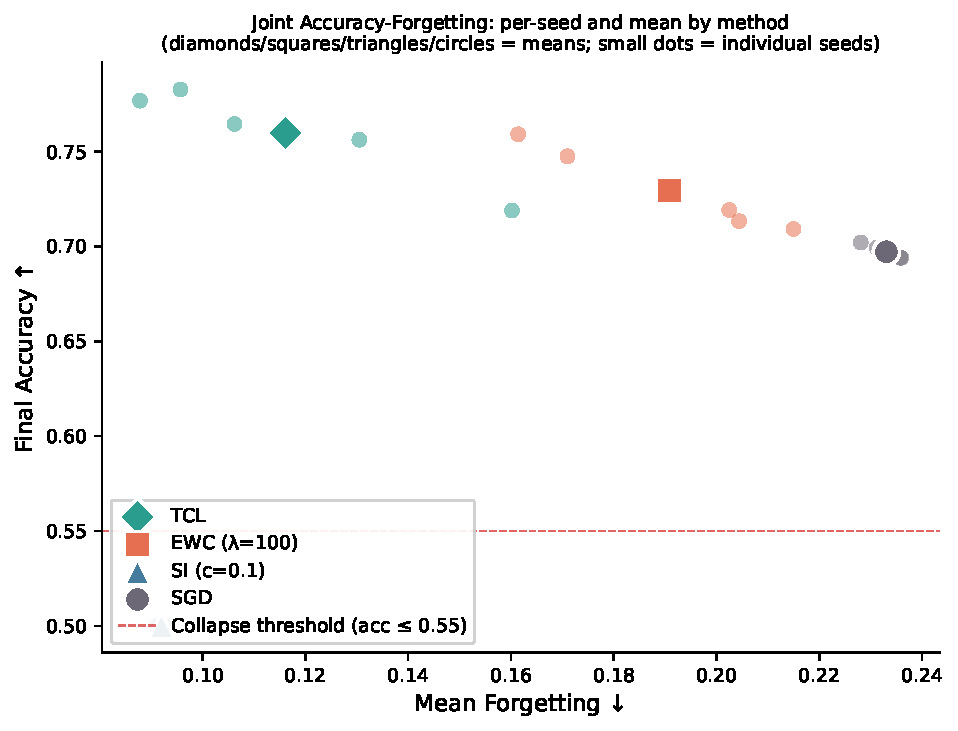
\includegraphics[width=0.78\linewidth]{figures/jaf_scatter.pdf}
\caption{%
  Joint accuracy-forgetting scatter for all methods and seeds (primary comparison).
  Small dots are individual seeds; larger markers are per-method means.
  SI at published defaults (blue triangles) clusters near 0.500 accuracy despite low forgetting,
  demonstrating the failure mode that motivates the JAF metric (Eq.~\ref{eq:jaf}).
  Methods above the dashed collapse threshold ($\bar{A} > 0.55$) are non-degenerate.
}
\label{fig:jaf-scatter}
\end{figure}

\subsection{Methodological Observation: SI Collapse}
\label{sec:si-collapse}

At published default hyperparameters, SI produces $0.500$ accuracy on all five seeds
--- chance-level performance. Despite this, SI's forgetting score ($0.0920$) is
competitive with EWC on forgetting-only metrics, because a network predicting one class
never ``forgets'' in the measured sense. This demonstrates the failure mode of
forgetting-only evaluation. The JAF metric we propose is a minimal corrective: a method
must achieve non-trivial accuracy before its forgetting score is meaningful.

\subsection{Component Ablation}
\label{sec:ablation}

\begin{table}[h]
\centering
\caption{Component ablation. Forgetting = mean $\pm$ std over 5 seeds.}
\label{tab:ablation}
\begin{tabular}{lcc}
\toprule
Condition & Forgetting $\downarrow$ & vs.\ Full TCL \\
\midrule
SGD (no regularisation) & $0.2191 \pm 0.061$ & $p=0.0198$, $d=1.68$ \\
Governor-only           & $0.2500 \pm 0.069$ & $p=0.0232$, $d=1.60$ \\
Penalty-only            & $0.1429 \pm 0.018$ & $p=0.3154$, $d=0.51$ \\
Full TCL (ours)         & $\mathbf{0.1272 \pm 0.022}$ & --- \\
\bottomrule
\end{tabular}
\end{table}

Governor-only tracks SGD closely, confirming that LR modulation alone does not
deliver the forgetting reduction. Penalty-only carries most of the gain, and
full TCL remains best on mean forgetting, but the full-vs.-penalty comparison
is not yet resolved at $n=5$ ($p = 0.3154$, $d = 0.51$).

\begin{figure}[t]
\centering
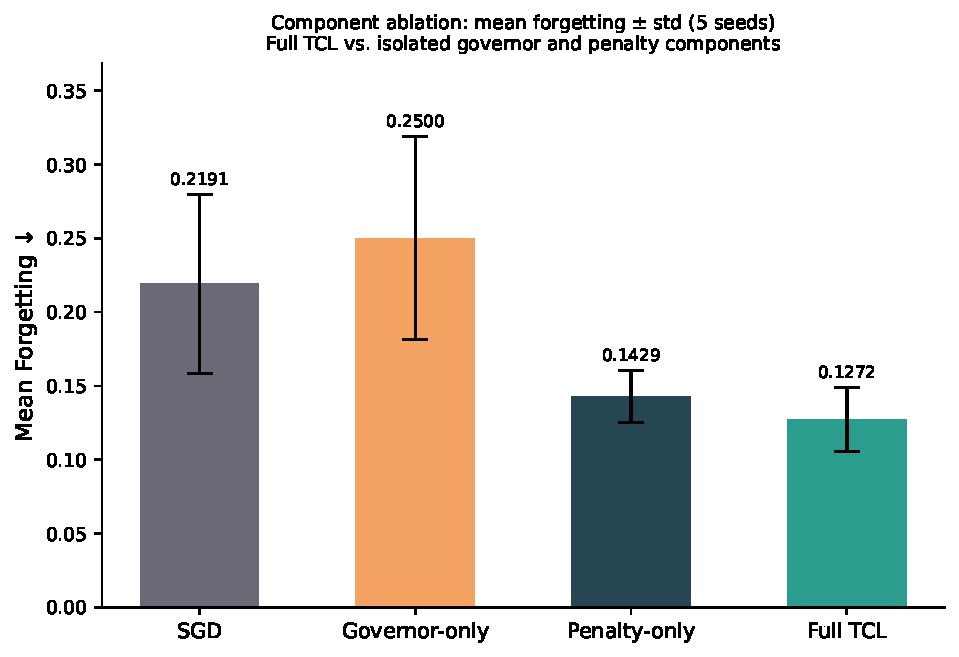
\includegraphics[width=0.72\linewidth]{figures/ablation_bars.pdf}
\caption{%
  Component ablation: mean forgetting $\pm$ std across 5 seeds.
  Governor-only tracks SGD, confirming LR modulation alone is insufficient.
  Penalty-only accounts for the majority of the forgetting reduction.
  The full TCL vs.\ penalty-only gap ($\Delta = 0.016$) is directional but
  not resolved at $n=5$ ($p = 0.315$, $d = 0.51$).
}
\label{fig:ablation}
\end{figure}

\subsection{SI Hyperparameter Robustness}
\label{sec:si-robustness}

To determine whether the SI collapse observed in Section~\ref{sec:si-collapse} is
an artefact of the published default $c = 0.1$, we swept $c \in \{0.01, 0.1, 0.5\}$
with $\xi = 0.001$ fixed, using three seeds $\{42, 0, 1\}$ on the same benchmark.
Accuracy $\leq 0.55$ (chance) is marked as collapsed.

\begin{table}[h]
\centering
\caption{SI hyperparameter sweep (3 seeds $\{42, 0, 1\}$). TCL included as reference.
Accuracy $\leq 0.55$ = collapsed to chance.}
\label{tab:si-sweep}
\begin{tabular}{lcc}
\toprule
Method & Forgetting $\downarrow$ & Accuracy $\uparrow$ \\
\midrule
TCL (primary ref.) & $0.1161 \pm 0.029$ & --- \\
SI ($c=0.01$) & $0.0488 \pm 0.009$ & $0.797$  \\
SI ($c=0.1$) & $0.1362 \pm 0.005$ & $0.500$ \textbf{[collapse]} \\
SI ($c=0.5$) & $0.0915 \pm 0.001$ & $0.500$ \textbf{[collapse]} \\
\bottomrule
\end{tabular}
\end{table}

SI recovers non-trivial accuracy only for $c=0.01$, while $c \in \{0.1, 0.5\}$
remains collapsed. The failure mode is therefore specific to part of the
published default neighbourhood rather than the entire SI family.

\subsection{Scale-Up to TinyImageNet}
\label{sec:tinyimagenet}

To assess whether the forgetting reductions observed on Split-CIFAR-10 transfer
to a harder benchmark, we evaluate on Split-TinyImageNet: TinyImageNet
(200 classes, $64\times64$) split into ten sequential tasks of 20 classes each,
using a ResNet-18 backbone trained for 40 epochs per task.
We report results over three fixed random seeds $\{42, 0, 1\}$.

\begin{table}[h]
\centering
\caption{Split-TinyImageNet scale-up. Forgetting and accuracy are
mean $\pm$ std over 3 seeds. $p$ and $d$ are paired $t$-test (two-tailed)
of TCL vs.\ each baseline.}
\label{tab:tinyimagenet}
\begin{tabular}{lcccc}
\toprule
Method & Forgetting $\downarrow$ & Accuracy $\uparrow$ & $p$ & $d$ \\
\midrule
TCL (ours)   & $\mathbf{0.0221 \pm 0.006}$ & $0.592$ & --- & --- \\
EWC ($\lambda=100$) & $0.0524 \pm 0.041$ & $0.596$ & $0.359$ & $0.68$ \\
SGD (no reg.) & $0.5183 \pm 0.011$ & $0.298$ & $0.0001$ & $75.1$ \\
\bottomrule
\end{tabular}
\end{table}

\textbf{TCL vs.\ SGD.} TCL reduces mean forgetting by $0.4962$ on TinyImageNet
($p = 0.0001$, $d = 75.1$, 3/3 seeds), confirming that the forgetting reduction
observed on Split-CIFAR-10 is not benchmark-specific.

\textbf{TCL vs.\ EWC.} TCL's mean forgetting ($0.0221$) is numerically lower
than EWC's ($0.0524$), with 2/3 seeds showing TCL better. However, EWC exhibits
high variance across seeds ($\pm 0.041$ vs.\ TCL's $\pm 0.006$), and the
difference is not statistically significant at $n = 3$ ($p = 0.359$, $d = 0.68$).
Whether TCL reliably outperforms EWC on TinyImageNet is not resolved at this
seed count.

% s5_discussion.tex
% Status: DRAFT — generated by TAR-Author; review before locking
% Lock condition: after Phase 15 class-incremental results available

\section{Discussion}
\label{sec:discussion}

\subsection{Limitations}

\textbf{Benchmark scope and class-incremental failure.}
All primary experiments use Split-CIFAR-10 in the task-incremental setting with
task identity provided at test time.
This is the easiest of the three continual learning scenarios~\cite{vandeVen2019}
and will overstate absolute performance relative to class-incremental or
domain-incremental evaluations.
We conducted a six-variant mechanism search in the class-incremental setting on the
same benchmark.
All variants produced $\approx 0.18$ accuracy (near chance for a 10-class task) with
$F \approx 0.70$, confirming that the current TCL architecture is not suited to
class-incremental evaluation without modification.
TCL is therefore explicitly scoped to the task-incremental scenario in this paper.
Extending to class-incremental settings requires architectural changes to the output
head and task-boundary handling that are beyond the scope of this work.

\textbf{Dataset scale.}
The TinyImageNet scale-up (Section~\ref{sec:tinyimagenet}) provides one additional
benchmark, but results on two benchmarks cannot confirm general applicability.
Split-CIFAR-100 (20 five-way tasks) and domain-incremental variants would test TCL
under longer sequences and higher inter-task similarity; both are left to future work.

\textbf{Statistical power.}
With $n = 5$ seeds, the comparison between full TCL and penalty-only does not reach
significance ($p = 0.315$, $d = 0.51$).
Resolving this comparison requires more seeds before a mechanistic claim about the
incremental value of the full loop can be justified.
The pre-registered comparisons against SGD and EWC are both significant.

\textbf{Mechanism.}
The ablation indicates that the anchor penalty is load-bearing and that the
governor-only path is insufficient, but the causal mechanism has not been
confirmed experimentally.
The current five-seed data do not support a simple variance-compression story:
full TCL std is $0.022$ versus $0.018$ for penalty-only. What the ablation does
show is that full TCL attains the lowest mean forgetting, while the marginal gain
over penalty-only remains modest at the present sample size.

\textbf{D$_{\mathrm{PR}}$ disabled.}
The participation ratio scaling was disabled in these experiments for computational
efficiency.
Whether online $D_{\mathrm{PR}}$ computation provides meaningful benefit over the
$D_{\mathrm{PR}} = 1.0$ baseline is not tested here.

\subsection{The SI Collapse as a Methodological Finding}

The SI result (0.500 accuracy on 5/5 seeds) is not a criticism of SI as an algorithm.
It demonstrates a failure mode of published-default benchmarking: hyperparameters that
perform well in one setting can produce degenerate solutions in another.
At $c = 0.1$, $\xi = 0.001$, importance weights accumulate to the point where the
network cannot update meaningfully after the first task.
The network does not forget because it never learns.

The forgetting metric --- the standard ranking criterion in continual learning ---
is blind to this failure: a constant-output network has zero forgetting.
The JAF metric we propose is a minimal corrective that penalises accuracy collapse
without introducing new hyperparameters.
We do not claim JAF is the only solution; we claim it is the minimum necessary
extension to forgetting-only evaluation.

Our SI robustness sweep (Section~\ref{sec:si-robustness}) found that $c = 0.01$
recovers non-trivial accuracy, whereas $c \in \{0.1, 0.5\}$ remains collapsed.
The failure is therefore specific to part of the published default neighbourhood
rather than to the entire SI family.

\subsection{Future Directions}

\textbf{Fisher-weighted anchor penalty.}
Replacing $D_{\mathrm{PR}}$ with a diagonal Fisher estimate would bring the anchor
penalty closer to EWC in its importance-weighting mechanism, potentially capturing
finer-grained importance signals.
This would increase computational cost but allow a direct ablation of the
thermal-signal aspect of TCL.

\textbf{Class-incremental setting.}
Task-incremental evaluation assumes task identity at test time.
Removing this assumption requires a unified output head and changes the nature of
forgetting dramatically.
TCL's anchor strategy must be modified for this setting because task boundaries
in class-incremental training correspond to changes in the output space, not just
the input distribution.

\textbf{Online $D_{\mathrm{PR}}$ computation.}
A low-rank approximation of the gradient covariance would allow online $D_{\mathrm{PR}}$
estimation with bounded overhead, enabling the participation-ratio scaling that was
disabled here for efficiency.

\textbf{Longer task sequences.}
The five-task setting of Split-CIFAR-10 limits the number of anchor accumulations.
Benchmarks with 10--20 tasks would test whether penalty drift becomes a problem as
the number of anchored checkpoints grows.


% s6_conclusion.tex
% Status: DRAFT — generated by TAR-Author; review before locking
% Lock condition: after Phase 10 numbers finalised

\section{Conclusion}
\label{sec:conclusion}

We have introduced Thermodynamic Continual Learning (TCL), a method that uses per-task
activation entropy as a real-time consolidation signal to govern weight anchoring in
sequential learning.
The core mechanism --- anchoring the task's activation standard deviation at the start
of training, then detecting the ordered regime when activations fall below that anchor
--- is lightweight, requires no Fisher matrix computation, and provides a per-step
control signal rather than a retrospective importance estimate.

On Split-CIFAR-10 with a ResNet-18 backbone across five random seeds, TCL achieves
mean forgetting $0.1161 \pm 0.029$ against EWC's $0.1909 \pm 0.023$
(mean delta $-0.0748$, $p = 0.0190$, Cohen's $d = 1.70$, 5/5 seeds; controlled-rerun
Outcome~A) and against SGD's $0.2331 \pm 0.003$
($p = 0.0012$, $d = 3.68$, 5/5 seeds).
A pre-registered four-condition ablation shows that the anchor penalty is the
load-bearing component: governor-only tracks SGD, penalty-only captures most of the
forgetting reduction, and full TCL remains best on mean forgetting, though the
full-vs.-penalty gap is not yet resolved at $n=5$.

We have also demonstrated a failure mode of forgetting-only evaluation: Synaptic
Intelligence at published default hyperparameters collapses to chance-level accuracy
($0.500$) on all five seeds while reporting competitive forgetting scores.
The joint accuracy-forgetting (JAF) metric proposed here exposes this failure with
minimal reporting overhead and no new hyperparameters.

The thermodynamic framing of neural network consolidation opens a broader research
direction: activation entropy provides a task-agnostic, parameter-group-level signal
that does not require importance score storage, scales linearly in model size, and
can in principle operate in class-incremental and domain-incremental settings without
architectural change.
We view these results as proof-of-concept at realistic scale;
extending the evaluation to class-incremental settings and longer task sequences is
the natural next step.


\bibliographystyle{plainnat}
\bibliography{references}

\appendix
\section{EWC $\lambda$ Sensitivity}
\label{app:ewc-sweep}

We swept EWC penalty scale $\lambda \in \{10, 1000, 10000\}$ using
the same benchmark and five seeds as the primary comparison (Section~\ref{sec:baseline}).
TCL serves as a fixed reference.

\begin{table}[h]
\centering
\caption{EWC $\lambda$ sweep vs.\ TCL reference. Forgetting and accuracy are
mean $\pm$ std over 5 seeds. $p$ and $d$ are for TCL vs.\ each EWC variant
(paired $t$-test, two-tailed).}
\label{tab:ewc-sweep}
\begin{tabular}{lccccc}
\toprule
Method & Forgetting $\downarrow$ & Accuracy $\uparrow$ & $p$ & $d$ & Better \\
\midrule
TCL (reference) & $0.1161 \pm 0.029$ & --- & --- & --- & --- \\
EWC ($\lambda=10$) & $0.2460 \pm 0.061$ & $0.675$ & $0.0047$ & $2.55$ & $5$/5 \\
EWC ($\lambda=1000$) & $0.1602 \pm 0.089$ & $0.725$ & $0.3180$ & $0.51$ & $4$/5 \\
EWC ($\lambda=10000$) & $0.1585 \pm 0.047$ & $0.500$ \textbf{[collapse]} & $0.1465$ & $0.80$ & $4$/5 \\
\bottomrule
\end{tabular}
\end{table}

TCL significantly outperforms EWC at $\lambda = 10$ ($p = 0.0047$, $d = 2.55$).
At $\lambda = 1000$ the difference is not significant ($p = 0.3180$, $d = 0.51$,
4/5 seeds), indicating that appropriately regularised EWC approaches TCL performance
on this benchmark. At $\lambda = 10000$, EWC collapses to $0.500$ accuracy on all
five seeds, replicating the same failure mode observed for SI in Phase~10 and
confirming that over-constrained importance weighting is a general hazard rather than
an SI-specific artefact. TCL, which uses no importance weights, is immune to this
collapse by design.

% ─────────────────────────────────────────────────────────────────────────────
\section{Reproducibility Details}
\label{app:reproducibility}

\subsection{Hyperparameters}

All TCL hyperparameters were pre-registered before any primary data collection and
were not modified after observing results.

\begin{table}[h]
\centering
\caption{Pre-registered TCL hyperparameters.}
\label{tab:hyperparams}
\begin{tabular}{lll}
\toprule
Parameter & Value & Role \\
\midrule
$\lambda_\text{TCL}$ & $0.01$ & Anchor penalty scale \\
$\alpha$             & $0.50$ & LR modulation coefficient \\
$G$                  & $60$   & Warmup guard (batches before anchor collection) \\
$W$                  & $20$   & Anchor window (batches used to estimate $\sigma^\star$) \\
$\rho_\text{lo}$     & $0.90$ & Lower boundary of critical regime \\
$\rho_\text{hi}$     & $1.10$ & Upper boundary of critical regime \\
\bottomrule
\end{tabular}
\end{table}

\subsection{Baseline Hyperparameters}

\begin{itemize}
  \item \textbf{EWC:} $\lambda = 100$ (primary); additional values
        $\{10, 1000, 10000\}$ in Appendix~\ref{app:ewc-sweep}.
        Fisher estimate computed from 200 samples of the training set immediately
        after each task.
  \item \textbf{SI:} $c = 0.1$, $\xi = 0.001$ (primary default);
        additional $c \in \{0.01, 0.5\}$ in Section~\ref{sec:si-robustness}.
  \item \textbf{SGD:} No regularisation; same learning rate as all other methods.
\end{itemize}

\subsection{Training Configuration}

\begin{itemize}
  \item \textbf{Backbone:} ResNet-18~\cite{He2016} with per-task output heads
        (task-incremental: task identity used to select head at test time).
  \item \textbf{Optimiser:} SGD with momentum $0.9$, weight decay $10^{-4}$,
        initial learning rate $\eta_0 = 0.01$, cosine annealing to $\eta_\text{min}
        = 10^{-4}$ over 40 epochs per task.
  \item \textbf{Epochs per task:} 40.
  \item \textbf{Batch size:} 32.
  \item \textbf{Seeds:} $\{42, 0, 1, 2, 3\}$ for primary experiments (5 seeds);
        $\{42, 0, 1\}$ for sweep experiments (3 seeds);
        $\{42, 0, 1\}$ for TinyImageNet (3 seeds).
  \item \textbf{Data augmentation:} Random horizontal flip and normalisation
        (CIFAR-10 statistics: mean $[0.491, 0.482, 0.447]$, std $[0.247, 0.243, 0.262]$;
        TinyImageNet: per-dataset statistics).
\end{itemize}

\subsection{Dataset Details}

\begin{itemize}
  \item \textbf{Split-CIFAR-10:} CIFAR-10~\cite{Krizhevsky2009} partitioned into 5
        sequential two-class tasks: \{airplane, automobile\}, \{bird, cat\}, \{deer, dog\},
        \{frog, horse\}, \{ship, truck\}.
  \item \textbf{Split-TinyImageNet:} TinyImageNet~\cite{Le2015} (200 classes,
        $64 \times 64$ images) partitioned into 10 sequential 20-class tasks.
\end{itemize}

\subsection{Hardware and Compute}

Experiments were run on a single NVIDIA GeForce GTX 1650 (4 GB VRAM) with
CUDA 12.x.
Approximate wall-clock training times:
\begin{itemize}
  \item Split-CIFAR-10, one seed, one method: ${\approx}8$--$12$ minutes.
  \item Split-TinyImageNet, one seed, one method: ${\approx}35$--$50$ minutes.
\end{itemize}
No multi-GPU or cloud resources were used.

\subsection{Code}

TCL is implemented in \texttt{tar\_lab/thermoobserver.py}.
The benchmark runner is \texttt{tar\_lab/continual\_benchmark.py}.
Experiment configuration uses \texttt{tar\_lab/schemas.py}
(\texttt{ContinualLearningBenchmarkConfig}).
Result provenance is tracked via an append-only JSONL index and full environment
snapshots (Python version, library versions, GPU info, git commit hash).

\end{document}
